Dopo l'esecuzione del programma di \verb|analytics.cpp|
ci vengono forniti i risultati dei dati.
Nella tabella \ref{tab:types} vengono forniti il numero di particelle generate per tipo. Si noti che non sono state contate le particelle generate da K$^*$.\\ Nell'istogramma in alto a sinistra della figura \ref{fig:canvas1} è possibile visualizzare tale distribuzione.

\begin{table}[htp]
    \centering
    \begin{tabular}{||c|c|c||}
        \hline \hline
        \multicolumn{3}{||c||}{\textsc{occorrenze}} \\
        \hline \hline
        tipo & osservate & attese \\
        \hline
        $\pi^+$ & $ (3998.0 \pm 2.0) \cdot 10^3$ & $4000 \cdot 10^3$\\
        $\pi^-$ & $ (3999.0 \pm 2.0) \cdot 10^3$ & $4000 \cdot 10^3$\\
        K$^+$ & $ (5002.5 \pm 7.1) \cdot 10^2$ & $5000 \cdot 10^2$\\
        K$^-$ & $ (5009.3 \pm 7.1) \cdot 10^2$ & $5000 \cdot 10^2$\\
        p$^+$ & $ (4509.9 \pm 6.7) \cdot 10^2$ & $4500 \cdot 10^2$\\
        p$^-$ & $ (4515.5 \pm 6.7) \cdot 10^2$ & $4500 \cdot 10^2$\\
        K$^*$ & $ (992.6 \pm 3.2) \cdot 10^2$ & $1000 \cdot 10^2$\\
        \textsc{tot} & $ (10000 \pm 3.2) \cdot 10^3$ & $10000 \cdot 10^3$\\
        \hline \hline 
    \end{tabular}
    \caption[\small Occorrenze delle particelle]{\small Numero di particelle osservate e attese per tipo di particella e quella totale (“\textsc{tot}"). NOTA: L'incertezza di \textsc{tot} è ottenuto per conteggio diretto del programma, non per propagazione degli errori.}
    \label{tab:types}
\end{table}

\begin{figure}[htbp]
    \centering
    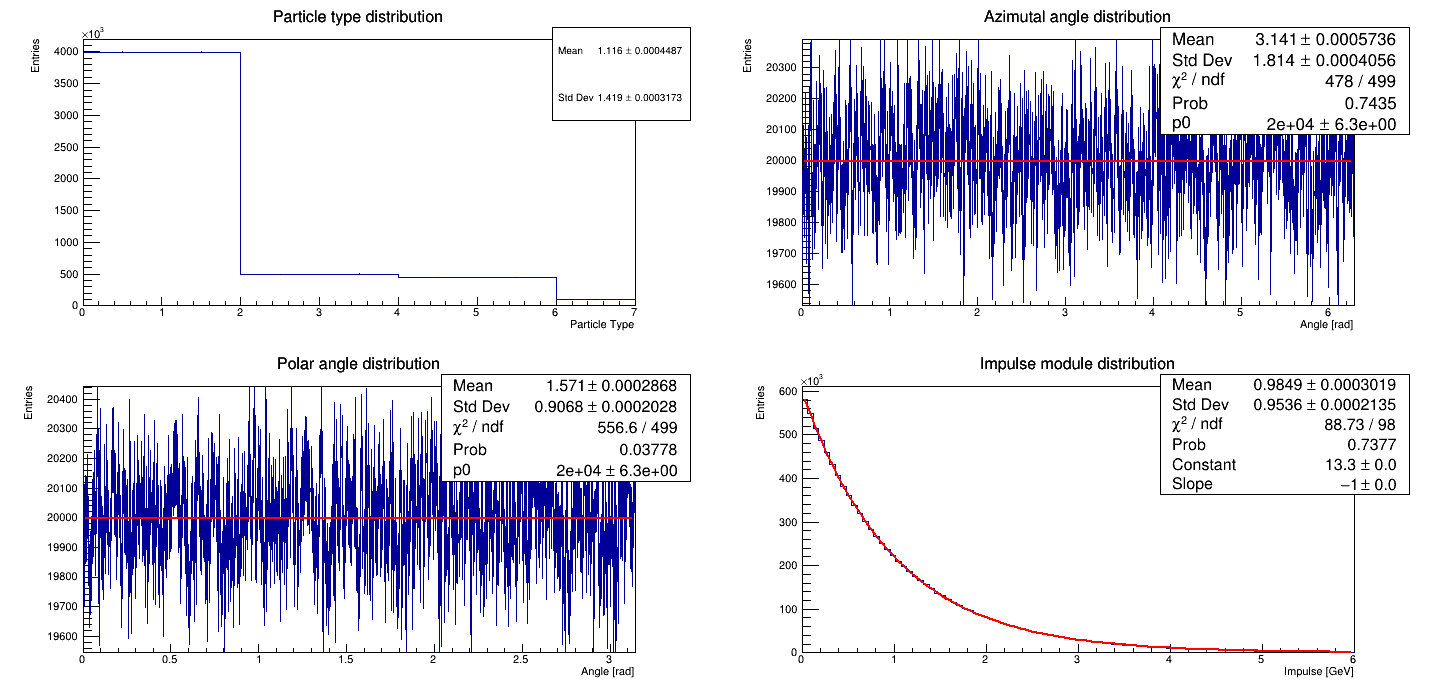
\includegraphics[width=\textwidth]{image/canvas1.png}
    \caption{\small Le distribuzioni rispettivamente (da sinistra a destra, da sopra a sotto) del numero di particelle per tipo, dell'angolo azimutale $\phi$, dell'angolo polare $\theta$ e dell'impulso. Se presenti, le curve rosse rappresentano il fit della funzione.}
    \label{fig:canvas1}
\end{figure}

In seguito nella tabella \ref{tab:ang_imp} si riportano i risultati relativi alla distribuzione dei fit degli angoli polari e azimutali e del modulo dell'impulso. In figura \ref{fig:canvas1} si osserva che le distribuzioni degli angoli sono uniformi, mentre la distribuzione dell'impulso è di decadimento esponenziale, come previsto nella sezione precedente.

\begin{table}[htp]
    \centering
    \begin{tabular}{||c|c|c|c|c||}
        \hline \hline
        \multicolumn{5}{||c||}{\textsc{analisi dei fit degli angoli $\phi$, $\theta$ e dell'impulso}} \\
        \hline \hline
        distribuzione & parametri & $\chi^2$ & DoF & $\chi^2/$DoF \\
        \hline
        angolo azimutale $\phi$ (unif.) & 19999.0 ± 6.3 & 477.97 & 499 & 0.957856\\
        angolo polare $\theta$ (unif.) & 19998.9 ± 6.3 & 556.553 & 499 & 1.11534\\
        modulo impulso (exp.) & 1.00019 ± 0.00033 & 88.7283 & 98 & 0.905391\\
        \hline \hline 
    \end{tabular}
    \caption[\small Distribuzione angoli e impulso]{\small Valori estratti dal fit delle distribuzioni dell'angolo azimutale $\phi$, dell'angolo polare $\theta$ e del modulo dell'impulso delle particelle generate.}
    \label{tab:ang_imp}
\end{table}

Nel prossimo passaggio il programma cerca di rilevare il segnale generato da K$^*$ dalle distribuzioni della massa invariante.\\
Per far ciò, vogliamo estrarre solo la massa invariante tra particelle generate da K$^*$ che sappiamo essere una coppia di K e $\pi$ di carica opposta. È possibile rilevare ciò facendo una differenza della distribuzione della massa invariante fra cariche discordi da quelle concordi, eliminando così il rumore generato tra combinazioni accidentali. Per aumentare l'efficienza della rilevazione basta sottrarre la distribuzione di masse invarianti di K e $\pi$ concordi da quelli discordi.\\
In tabella \ref{tab:massinv} si trovano i risultati dei fit di queste differenze, messa in confronto con la distribuzione di massa invariante facente da benchmark, che rappresenta la distribuzione migliore del segnale di K$^*$. Si nota come i valori della media e del sigma si avvicinano rispettivamente ai valori della massa e della larghezza di risonanza di K$^*$. Si possono inoltre visualizzare queste distribuzioni in figura \ref{fig:canvas2}.

\begin{table}[htp]
    \centering
    \begin{tabular}{||c|c|c|c|c||}
        \hline \hline
        \multicolumn{5}{||c||}{\textsc{analisi del fit di K$^*$}} \\
        \hline \hline
        distribuzione & media & sigma & ampiezza & $\chi^2/$DoF \\
        \hline
        massa inv. best & 0.89155 ± 0.00016 & 0.05084 ± 0.00012 & 23363 ± 91 & 1.47239\\
        massa inv. totale & 0.887 ± 0.011 & 0.0349 ± 0.0098 & (10.1 ± 2.4) $\cdot 10^3$ & 0.859503\\
        massa inv. K e $\pi$ & 0.8778 ± 0.0080 & 0.0443 ± 0.0070 & (7.4 ± 1.1) $\cdot 10^3$ & 0.827187\\
        \hline \hline 
    \end{tabular}
    \caption[\small Distribuzioni massa invariante]{\small Valori estratti dal fit delle distribuzioni della massa invariante migliore (“best"), della differenza tra cariche discordi e quelli concordi (“totale") e della differenza tra K e $\pi$ di carica discorde e concorde (“K e $\pi$").}
    \label{tab:massinv}
\end{table}

\begin{figure}[htbp]
    \centering
    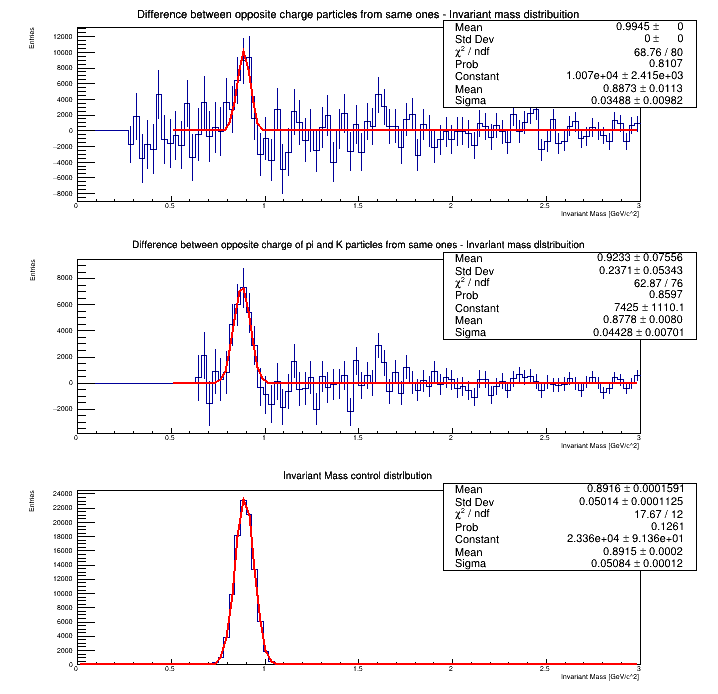
\includegraphics[width=.8\textwidth]{image/canvas2.png}
    \caption{\small Le distribuzioni rispettivamente della differenza della massa invariante tra particelle di carica opposta e concorde, tra K e $\pi$ di carica opposta e concorde e infine della differenza di massa invariante migliore.}
    \label{fig:canvas2}
\end{figure}